%% abtex2-modelo-trabalho-academico.tex, v-1.9.2 laurocesar
%% Copyright 2012-2014 by abnTeX2 group at http://abntex2.googlecode.com/ 
%%
%% This work may be distributed and/or modified under the
%% conditions of the LaTeX Project Public License, either version 1.3
%% of this license or (at your option) any later version.
%% The latest version of this license is in
%%   http://www.latex-project.org/lppl.txt
%% and version 1.3 or later is part of all distributions of LaTeX
%% version 2005/12/01 or later.
%%
%% This work has the LPPL maintenance status `maintained'.
%% 
%% The Current Maintainer of this work is the abnTeX2 team, led
%% by Lauro César Araujo. Further information are available on 
%% http://abntex2.googlecode.com/
%%
%% This work consists of the files abntex2-modelo-trabalho-academico.tex,
%% abntex2-modelo-include-comandos and abntex2-modelo-references.bib
%%

% ------------------------------------------------------------------------
% ------------------------------------------------------------------------
% abnTeX2: Modelo de Trabalho Academico (tese de doutorado, dissertacao de
% mestrado e trabalhos monograficos em geral) em conformidade com 
% ABNT NBR 14724:2011: Informacao e documentacao - Trabalhos academicos -
% Apresentacao
% ------------------------------------------------------------------------
% ------------------------------------------------------------------------

%-------------------------------------------------------------------------
% Modelo adaptado especificamente para o contexto do PPgSI-EACH-USP por 
% Marcelo Fantinato, com auxílio dos Professores Norton T. Roman, Helton
% H. Bíscaro e Sarajane M. Peres, em 2015, com muitos agradecimentos aos 
% criadores da classe e do modelo base.
%
% 20/06/2017: inclusão de "lista de quadros" com base no especificado em:
% https://github.com/abntex/abntex2/wiki/HowToCriarNovoAmbienteListing,
% de autoria de "Eduardo de Santana Medeiros Alexandre".
%
%-------------------------------------------------------------------------

\documentclass[
	% -- opções da classe memoir --
	12pt,				% tamanho da fonte
	% openright,			% capítulos começam em pág ímpar (insere página vazia caso preciso)
	oneside,			% para impressão apenas no anverso (apenas frente). Oposto a twoside
	a4paper,			% tamanho do papel. 
	% -- opções da classe abntex2 --
	%chapter=TITLE,		% títulos de capítulos convertidos em letras maiúsculas
	%section=TITLE,		% títulos de seções convertidos em letras maiúsculas
	%subsection=TITLE,	% títulos de subseções convertidos em letras maiúsculas
	%subsubsection=TITLE,% títulos de subsubseções convertidos em letras maiúsculas
	% -- opções do pacote babel --
	english,			% idioma adicional para hifenização
	%french,				% idioma adicional para hifenização
	%spanish,			% idioma adicional para hifenização
	brazil				% o último idioma é o principal do documento
	]{abntex2ppgsi}

% ---
% Pacotes básicos 
% ---
% \usepackage{lmodern}			% Usa a fonte Latin Modern			
% \usepackage[T1]{fontenc}		% Selecao de codigos de fonte.
\usepackage[utf8]{inputenc}		% Codificacao do documento (conversão automática dos acentos)
\usepackage{lastpage}			% Usado pela Ficha catalográfica
\usepackage{indentfirst}		% Indenta o primeiro parágrafo de cada seção.
\usepackage{color}				% Controle das cores
\usepackage{graphicx}			% Inclusão de gráficos
\usepackage{microtype} 			% para melhorias de justificação
\usepackage{pdfpages}     %para incluir pdf
\usepackage{algorithm}			%para ilustrações do tipo algoritmo
\usepackage{mdwlist}			%para itens com espaço padrão da abnt
\usepackage[noend]{algpseudocode}			%para ilustrações do tipo algoritmo
\usepackage{chemformula} % para escrever CO2 corretamente
\usepackage{longtable} % para tab elas longas
		
% ---
% Pacotes adicionais, usados apenas no âmbito do Modelo Canônico do abnteX2
% ---
\usepackage{lipsum}				% para geração de dummy text
% ---

% ---
% Pacotes de citações
% ---
\usepackage{hyperref}
\usepackage[brazilian,hyperpageref]{backref}	 % Paginas com as citações na bibl
\usepackage[alf,abnt-etal-list=0,abnt-etal-text=it]{abntex2cite}	% Citações padrão ABNT

% --- 
% CONFIGURAÇÕES DE PACOTES
% --- 

% ---
% Configurações do pacote backref
% Usado sem a opção hyperpageref de backref
\renewcommand{\backrefpagesname}{Citado na(s) página(s):~}
% Texto padrão antes do número das páginas
\renewcommand{\backref}{}
% Define os textos da citação
\renewcommand*{\backrefalt}[4]{
	\ifcase #1 %
		Nenhuma citação no texto.%
	\or
		Citado na página #2.%
	\else
		Citado #1 vezes nas páginas #2.%
	\fi}%
% ---

% ---
% Informações de dados para CAPA e FOLHA DE ROSTO
% ---
\instituicao{
	UNIVERSIDADE DE SÃO PAULO
	\par
	ESCOLA DE ARTES, CIÊNCIAS E HUMANIDADES
	\par
	PROGRAMA DE PÓS-GRADUAÇÃO EM SISTEMAS DE INFORMAÇÃO}

%-------------------------------------------------------------------------
% Comentário adicional do PPgSI - Informações sobre o ``título'':
%
% Em maiúscula apenas a primeira letra da sentença (do título), exceto 
% nomes próprios, geográficos, institucionais ou Programas ou Projetos ou 
% siglas, os quais podem ter letras em maiúscula também.
%
% O subtítulo do trabalho é opcional.
% Sem ponto final.
%
% Atenção: o título da Dissertação/Tese na versão corrigida não pode mudar. 
% Ele deve ser idêntico ao da versão original.
%
%-------------------------------------------------------------------------
\titulo{Estratégias de migração de máquinas virtuais para a redução da pegada de carbono na computação em nuvem verde}
\autor{\uppercase{Guilherme Fernandes Moraes da Silva}}
\local{São Paulo}

%-------------------------------------------------------------------------
% Comentário adicional do PPgSI - Informações sobre a ``data'':
%
% Colocar o ano do depósito (ou seja, o ano da entrega) da respectiva 
% versão, seja ela a versão original (para a defesa) seja ela a versão 
% corrigida (depois da aprovação na defesa). 
%
% Atenção: Se a versão original for depositada no final do ano e a versão 
% corrigida for entregue no ano seguinte, o ano precisa ser atualizado no 
% caso da versão corrigida. 
% Cuidado, pois o ano da ``capa externa'' também precisa ser atualizado 
% nesse caso.
%
% Não incluir o dia, nem o mês.
% Sem ponto final.
%-------------------------------------------------------------------------
\data{2024}
\orientador{Prof. Dr. Daniel de Angelis Cordeiro}
\tipotrabalho{Dissertação (Mestrado) / Tese (Doutorado)}

\preambulo{
Projeto de pesquisa para exame de qualificação apresentado à Escola de Artes, Ciências e Humanidades da Universidade de São Paulo como parte dos requisitos para obtenção do título de Mestre em Ciências pelo Programa de Pós-graduação em Sistemas de Informação.
\newline \newline Área de concentração: Metodologia e Técnicas da Computação
}

% ---
% Configurações de aparência do PDF final

% alterando o aspecto da cor azul
\definecolor{blue}{RGB}{41,5,195}

% informações do PDF
\makeatletter
\hypersetup{
     	%pagebackref=true,
		pdftitle={\@title}, 
		pdfauthor={\@author},
    	pdfsubject={\imprimirpreambulo},
	    pdfcreator={laTeX com abnTeX2 adaptado para o PPgSI-EACH-USP},
		pdfkeywords={abnt}{latex}{abntex}{abntex2ppgsi}{qualificação de mestrado}{dissertação de mestrado}{qualificação de doutorado}{tese de doutorado}{ppgsi}, 
		colorlinks=true,       		% false: boxed links; true: colored links
    	linkcolor=blue,          	% color of internal links
    	citecolor=blue,        		% color of links to bibliography
    	filecolor=magenta,      		% color of file links
		urlcolor=blue,
		bookmarksdepth=4
}
\makeatother
% --- 

% --- 
% Espaçamentos entre linhas e parágrafos 
% --- 

% O tamanho do parágrafo é dado por:
\setlength{\parindent}{1.25cm}

% Controle do espaçamento entre um parágrafo e outro:
\setlength{\parskip}{0cm}  % tente também \onelineskip
\renewcommand{\baselinestretch}{1.5}

% ---
% compila o indice
% ---
\makeindex
% ---

	% Controlar linhas orfas e viuvas
  \clubpenalty10000
  \widowpenalty10000
  \displaywidowpenalty10000

% ----
% Início do documento
% ----
\begin{document}

% Retira espaço extra obsoleto entre as frases.
\frenchspacing 

% ----------------------------------------------------------
% ELEMENTOS PRÉ-TEXTUAIS
% ----------------------------------------------------------
% \pretextual

% ---
% Capa
% ---
%-------------------------------------------------------------------------
% Comentário adicional do PPgSI - Informações sobre a ``capa'':
%
% Esta é a ``capa'' principal/oficial do trabalho, a ser impressa apenas 
% para os casos de encadernação simples (ou seja, em ``espiral'' com 
% plástico na frente).
% 
% Não imprimir esta ``capa'' quando houver ``capa dura'' ou ``capa brochura'' 
% em que estas mesmas informações já estão presentes nela.
%
%-------------------------------------------------------------------------
\imprimircapa
% ---

% ---
% Folha de rosto
% (o * indica que haverá a ficha bibliográfica)
% ---
\imprimirfolhaderosto*
% ---

% ---
% ---
% inserir lista de figuras
% ---
\pdfbookmark[0]{\listfigurename}{lof}
\listoffigures*
\cleardoublepage
% ---

% ---
% inserir lista de abreviaturas e siglas
% ---
%-------------------------------------------------------------------------
% Comentário adicional do PPgSI - Informações sobre ``Lista de abreviaturas 
% e siglas'': 
%
% Opcional.
% Uma vez que se deseja usar, é necessário manter padrão e consistência no
% trabalho inteiro.
% Se usar: inserir em ordem alfabética.
%
%-------------------------------------------------------------------------
\begin{siglas}
  \item[CRC] \textit{Carbon-responsive computing}
  \item[IaaS] \textit{Infrastructure as a Service}
  \item[PaaS] \textit{Platform as a Service}
  \item[SaaS] \textit{Software as a Service}
  \item[TI] Tecnologia da informação
  \item[VM] Máquina virtual
  \item[VMM] Monitor de máquina virtual
\end{siglas}
% ---


% ---
% inserir lista de símbolos
% ---
%-------------------------------------------------------------------------
% Comentário adicional do PPgSI - Informações sobre ``Lista de símbolos'': 
%
% Opcional.
% Uma vez que se deseja usar, é necessário manter padrão e consistência no
% trabalho inteiro.
% Se usar: inserir na ordem em que aparece no texto.
% 
%-------------------------------------------------------------------------
\begin{simbolos}
	\item[$ \alpha $] Letra grega minúscula Alfa
	\item[$ \beta $] Letra grega minúscula Beta
	\item[$ \gamma $] Letra grega minúscula Gama
  \end{simbolos}
  % ---

% ---
% inserir o sumario
% ---
\pdfbookmark[0]{\contentsname}{toc}
\tableofcontents*
\cleardoublepage
% ---



% ----------------------------------------------------------
% ELEMENTOS TEXTUAIS
% ----------------------------------------------------------
\textual



%-------------------------------------------------------------------------
% Comentário adicional do PPgSI - Informações sobre ``títulos de seções''
% 
% Para todos os títulos (seções, subseções, tabelas, ilustrações, etc.):
%
% Em maiúscula apenas a primeira letra da sentença (do título), exceto 
% nomes próprios, geográficos, institucionais ou Programas ou Projetos ou
% siglas, os quais podem ter letras em maiúscula também.
%
%-------------------------------------------------------------------------
\chapter{Introdução}

\section{Contextualização}

\section{Justificativa}

\section{Problema de pesquisa}

\section{Proposição de pesquisa}

\section{Objetivos}

\subsection{Objetivos gerais}

\subsection{Objetivos específicos}

\section{Método de pesquisa}

\section{Cronograma proposto}

\section{Limitações e riscos}

\section{Estrutura do documento}

\chapter{Fundamentação teórica}\label{chapter:fundamentacao-teorica}

Neste capítulo são apresentados conceitos fundamentais para o leitor entender os demais capítulos desta dissertação. Primeiro, os conceitos de máquinas virtuais e migração de máquinas virtuais são apresentados na Seção \ref{section:maquinas-virtuais}. Em seguida, a Seção \ref{section:computacao-nuvem} apresenta os conceitos de computação em nuvem e computação em nuvem verde, além de fornecer uma visão geral sobre esses temas atualmente. Por fim, a Seção \ref{section:escalonamento} introduz o conceito de escalonamento e como ele é utilizado no contexto de computação em nuvem.

\section{Máquinas Virtuais}\label{section:maquinas-virtuais}

Uma máquina virtual (VM) é um ambiente virtualizado criado pelo hipervisor, também conhecido como monitor de máquina virtual (VMM). O VMM gerencia os recursos físicos do sistema anfitrião (a máquina física) e provisiona múltiplos ambientes virtuais independentes, chamados de convidados. Sua função principal é garantir que essas VMs compartilhem os recursos físicos de forma eficiente, evitando, por exemplo, que a mesma região de memória seja alocada simultaneamente para mais de uma VM. Dessa forma, a VM atua como uma duplicata isolada e eficiente de uma máquina real, permitindo a execução de sistemas operacionais e aplicações de forma independente e segura \cite{10.1145/361011.361073}.

Entre a máquina física e as VMs, há uma camada de software que possibilita a virtualização dos recursos. Essa camada, controlada pelo VMM, permite que as VMs superem as limitações de compatibilidade de hardware e recursos, criando um ambiente mais flexível. Em sistemas tradicionais de virtualização, o VMM opera com os mais altos privilégios, enquanto as VMs funcionam com privilégios reduzidos. Isso garante que o hipervisor possa interceptar e controlar ações que, de outra forma, acessariam ou modificariam componentes críticos do hardware, assegurando o isolamento entre as VMs e a estabilidade do sistema anfitrião. Com essa separação, torna-se possível executar diversos sistemas operacionais ou aplicações simultaneamente em uma única máquina física, o que maximiza o uso dos recursos e melhora a eficiência do ambiente computacional \cite{1430629}.

A implementação de tecnologias de virtualização também relaxa as restrições impostas pelo \textit{hardware}, e amplia a flexibilidade do sistema. A virtualização oferece um ambiente abstrato e isolado para a execução de aplicações, o que permite maior escalabilidade e facilita o gerenciamento de recursos. Além disso, existe um vasto conjunto de tecnologias e conceitos que tornam essa abstração possível, proporcionando uma infraestrutura mais adaptável às demandas dinâmicas da computação moderna \cite{10.5555/2531413}.

\subsection{Migração ao vivo de Máquinas Virtuais}\label{section:migracao-ao-vivo-maquinas-virtuais}

A migração ao vivo de máquinas virtuais é um processo útil para a administração de \textit{data centers} e \textit{clusters}, pois separa o \textit{hardware} do \textit{software}, o que facilita o gerenciamento de falhas, balanceamento de carga e manutenção. Ao transferir o sistema operacional e suas aplicações como uma unidade, esse processo permite mover o estado em memória de forma eficiente e consistente, garantindo a continuidade da execução sem interrupções. Uma das principais vantagens dessa abordagem é a possibilidade de desativar a máquina original após a conclusão da migração, o que é especialmente útil para realizar a manutenção do \textit{hardware}. Ao migrar a máquina virtual completa, o processo ocorre de forma transparente para os serviços em execução, eliminando a necessidade de gerenciar detalhes internos da VM. Isso permite, por exemplo, a migração de servidores de jogos \textit{online} sem desconectar os usuários, algo inviável em métodos que dependem da reinicialização no nível da aplicação ou do redirecionamento na camada de aplicação \cite{10.5555/1251203.1251223}.

\section{Computação em nuvem}\label{section:computacao-nuvem}

A computação em nuvem surgiu como uma solução para um dos maiores desafios da indústria tecnológica: a necessidade de que usuários e empresas adquirissem e mantivessem sua própria infraestrutura para disponibilizar serviços e aplicações. Com o crescimento exponencial da \textit{internet}, a tarefa de escalar essa infraestrutura para atender à demanda crescente tornou-se cada vez mais complexa e custosa. Conforme \citeonline{4738445}, a computação em nuvem pode ser definida como um paradigma de computação distribuída em larga escala, impulsionado pelas economias de escala, no qual um conjunto de recursos --- como computação, armazenamento, plataformas e serviços --- é abstraído, virtualizado, escalonável dinamicamente e gerenciado para ser entregue sob demanda a clientes externos por meio da \textit{internet}.

Dentro desse paradigma, as plataformas de computação em nuvem geralmente oferecem serviços em três diferentes níveis: IaaS (\textit{Infrastructure as a Service}), PaaS (\textit{Platform as a Service}) e SaaS (\textit{Software as a Service}), como descrito por \citeonline{4738445}. No nível IaaS, a plataforma fornece aos usuários acesso a recursos de \textit{hardware}, como processamento e armazenamento, cobrando de acordo com a utilização. Exemplos de serviços nesse nível incluem o Amazon EC2 (\textit{Elastic Cloud Computing}) e o Amazon S3 (\textit{Simple Storage Service}). No nível PaaS, o provedor oferece um ambiente completo para desenvolvimento, teste e implantação de aplicações, exigindo que os desenvolvedores sigam um modelo de desenvolvimento predefinido, aceitando algumas restrições em troca da escalabilidade oferecida, como no caso do Azure App Service. Por fim, no nível SaaS, aplicações específicas são disponibilizadas aos usuários por meio da \textit{internet}, com a cobrança proporcional ao uso do aplicativo. Exemplos incluem o Google Drive e o YouTube.

As plataformas modernas de computação em nuvem são compostas por diversos \textit{data centers} geodistribuídos. A Figura \ref{fig:microsoft-datacenters}, por exemplo, ilustra as localizações dos \textit{data centers} da Azure, da Microsoft, que somam milhões de servidores físicos \citeonline{john_roach_2021_microsoft_azure}. Essa infraestrutura geodistribuída é fundamental para atender à crescente demanda global de usuários, além de reduzir significativamente o tempo de resposta das aplicações, uma vez que a proximidade física dos servidores em relação aos usuários finais melhora a latência. A geodistribuição também oferece vantagens em termos de segurança e redundância. Se um \textit{data center} em uma determinada região ficar indisponível devido a falhas de energia, desastres naturais ou ataques cibernéticos, outro \textit{data center} em uma região distinta pode assumir temporariamente a carga computacional, assegurando a continuidade dos serviços.

\begin{figure}[htbp]
	\centering
	\caption{Localizações geográficas dos \textit{data centers} da Microsoft Azure}
		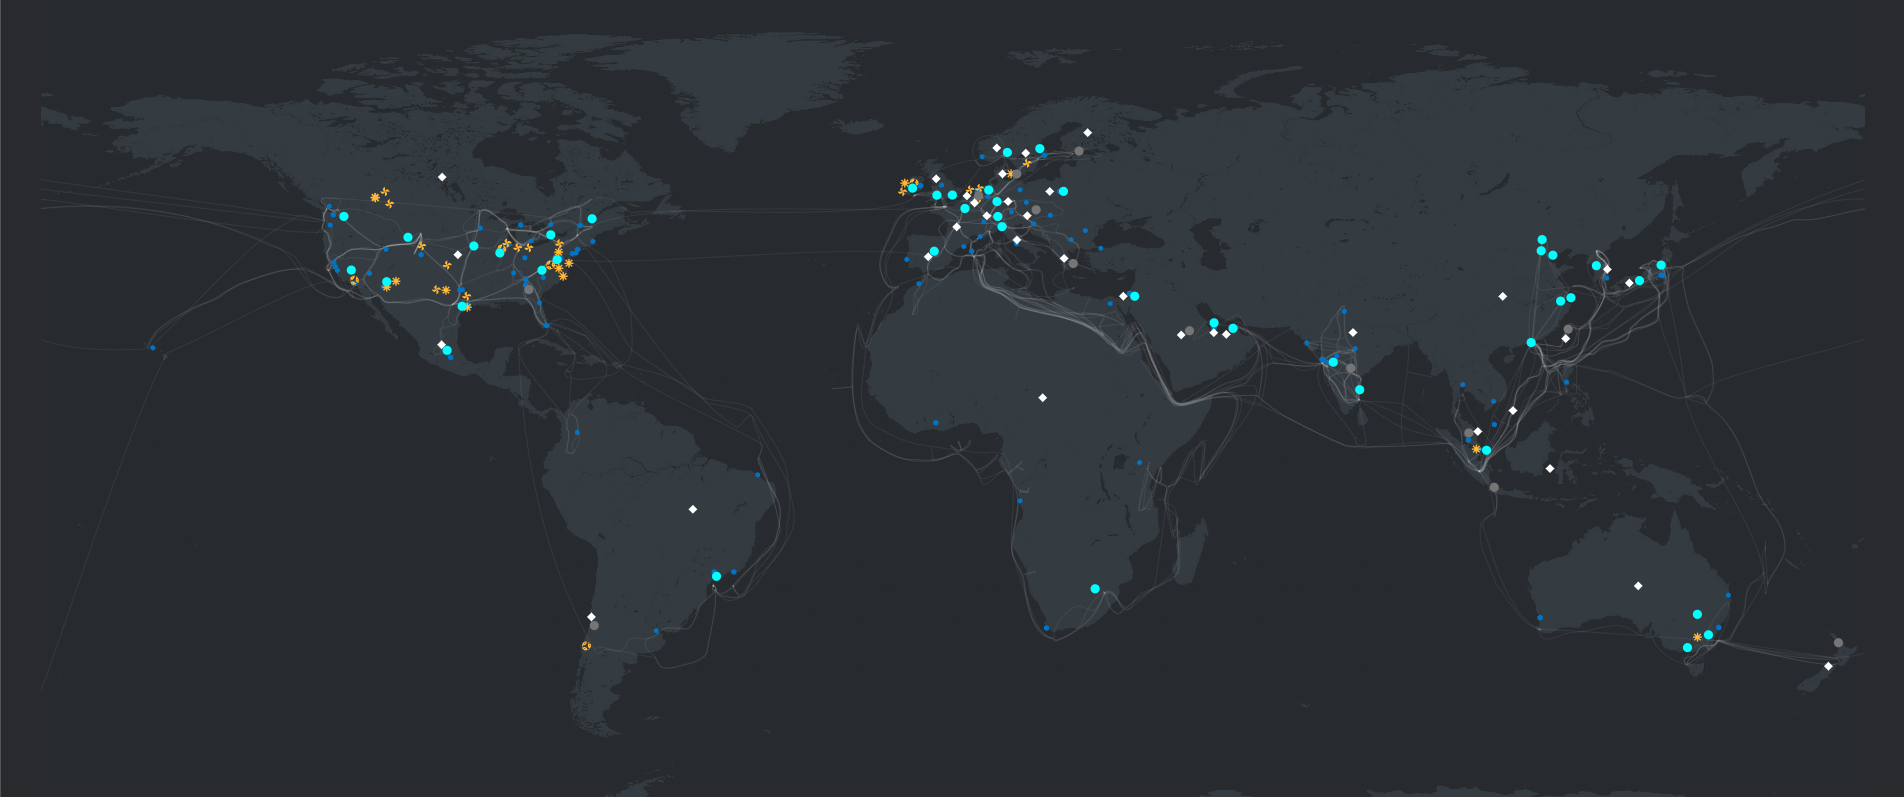
\includegraphics[width=\linewidth]{images/microsoft-datacenters.png}
	\label{fig:microsoft-datacenters}
  \source{\citeonline{azure_data_centers_locations}}
\end{figure}

\subsection{Computação em nuvem verde}

A computação verde é um paradigma que visa a criação de soluções tecnológicas ambientalmente sustentáveis e energeticamente eficientes. Esse conceito envolve o planejamento e o desenvolvimento de infraestruturas de computação e estratégias baseadas em princípios de gestão ambiental, otimização do consumo energético e práticas de reutilização. O objetivo central é promover a criação de produtos e serviços de tecnologia da informação (TI) que demandem menos energia e emitam menores quantidades de carbono. Nesse sentido, a computação verde busca reduzir o consumo de energia enquanto melhora a utilização da infraestrutura computacional, assegurando a expansão sustentável da computação em nuvem no longo prazo \cite{9793067}.

Em paralelo a esses esforços, tanto a academia quanto a indústria têm desenvolvido iniciativas para mitigar o impacto ambiental da computação em larga escala. Uma dessas iniciativas é o conceito de \textit{carbon-responsive computing} (CRC), que foca na priorização do uso de fontes de energia com menor intensidade de carbono, seja por meio de estratégias espaciais, temporais ou uma combinação de ambas. O CRC organiza-se em três estágios sequenciais, nos quais o progresso de cada fase depende da implementação adequada da anterior \cite{en14216917}.

O primeiro estágio, denominado \textit{carbon-aware computing}, compreende sistemas capazes de caracterizar e prever a intensidade de carbono, bem como medir o consumo energético associado. No segundo estágio, \textit{carbon-responsive computing}, as ações do sistema são orientadas pela intensidade de carbono em uso, ajustando o consumo energético conforme os níveis de emissões. Por fim, o terceiro estágio, \textit{carbon-resilient computing}, aborda a gestão e integração de elementos responsivos ao carbono, investigando as modificações necessárias nas infraestruturas de TI e de energia para reduzir a pegada de carbono e garantir maior resiliência ambiental \cite{en14216917}.

No contexto da infraestrutura geodistribuída da computação em nuvem, um dos principais mecanismos que permitem a implementação dessas estratégias ambientais é a migração ao vivo de máquinas virtuais, apresentada na Seção \ref{section:migracao-ao-vivo-maquinas-virtuais}. Como mencionado anteriormente, essa técnica possibilita a transferência de cargas de trabalho entre diferentes \textit{data centers} sem interrupções no serviço, promovendo o balanceamento de carga de maneira eficiente. Ao redirecionar o processamento para regiões onde a pegada de carbono é menor ou onde há disponibilidade de fontes de energia renováveis, a migração ao vivo contribui significativamente para a redução do impacto ambiental da computação em nuvem. Esse processo não só melhora a eficiência energética dos \textit{data centers}, como também apoia diretamente os objetivos de mitigação das emissões de carbono, e reforça o compromisso da computação verde com a sustentabilidade.

\section{Escalonamento}\label{section:escalonamento}

O escalonamento de tarefas é um desafio de otimização combinatória, no qual, dadas as características de um conjunto de recursos computacionais ($\alpha$) e de um conjunto de tarefas ($\beta$), o objetivo é encontrar uma alocação de recursos em tempo que minimize algum critério de otimização ($\gamma$). Essa formulação é frequentemente expressa pela notação \mbox{$\alpha$ $\vert$ $\beta$ $\vert$ $\gamma$}, introduzida por \citeonline{GRAHAM1979287}. Em ambientes de computação em nuvem, esses problemas de escalonamento ganham relevância à medida que a demanda por recursos computacionais cresce, exigindo alocações eficientes e dinâmicas que atendam a critérios como desempenho, economia de energia e sustentabilidade.

Um dos principais critérios de otimização nesse contexto é o \textit{makespan} ($C_{\max}$), que define o tempo em que a última tarefa de uma aplicação finaliza sua execução. Quando os recursos computacionais disponíveis são idênticos e conhecidos previamente, e o objetivo é minimizar o \textit{makespan} --- uma situação típica em problemas de escalonamento em \textit{clusters} --- o problema se torna fortemente NP-completo. Esse tipo de problema é denotado como $P\,\vert\,\vert\,C_{\max}$ \cite{GRAHAM1979287}.

No contexto desta dissertação, $\alpha$ representa os recursos computacionais disponíveis nos servidores dos \textit{data centers}, além de informações sobre a disponibilidade de fontes de energia com menor intensidade de carbono. Já $\beta$ descreve as exigências das VMs, como tempo de execução, prazos, memória e CPU. O critério $\gamma$ é a minimização do consumo de energia proveniente de fontes com alta intensidade de carbono, o que se alinha ao conceito de computação verde.

\chapter{Trabalhos correlatos}\label{chapter:trabalhos-correlatos}

% ----------------------------------------------------------
% ELEMENTOS PÓS-TEXTUAIS
% ----------------------------------------------------------
\postextual
% ----------------------------------------------------------

% ----------------------------------------------------------
% Referências bibliográficas
% ----------------------------------------------------------
\bibliography{referencias}

% ----------------------------------------------------------
% Glossário
% ----------------------------------------------------------
%
% Consulte o manual da classe abntex2 para orientações sobre o glossário.
%
%\glossary

% ----------------------------------------------------------
% Apêndices
% ----------------------------------------------------------

% ---
% Inicia os apêndices
% ---
\begin{apendicesenv}

% Imprime uma página indicando o início dos apêndices
%\partapendices

%-------------------------------------------------------------------------
% Comentário adicional do PPgSI - Informações sobre ``apêndice''
%
% Para todos os captions/(títulos) (de seções, subseções, tabelas, 
% ilustrações, etc.):
%     - em maiúscula apenas a primeira letra da sentença (do título), 
%       exceto nomes próprios, geográficos, institucionais ou Programas ou
%       Projetos ou siglas, os quais podem ter letras em maiúscula também.
%
% Todas  as tabelas, ilustrações (figuras, quadros, gráficos etc. ), 
% anexos, apêndices devem obrigatoriamente ser citados no texto.
%      - a citação deve vir sempre antes da primeira vez em que a tabela, 
%        ilustração etc., aparecer pela primeira vez.
%
%-------------------------------------------------------------------------
\chapter{Protocolo da revisão do estado da arte}

\section{Tema da revisão}\label{section:tema-da-revisao}

A revisão aborda a otimização da migração de VMs em \textit{data centers} geodistribuídos, com o propósito de minimizar o impacto ambiental e melhorar a eficiência operacional. O foco é reduzir as emissões de \ch{CO2}, o \textit{downtime} das aplicações e o congestionamento de rede, além de otimizar o uso de fontes de energia de baixa intensidade de carbono. A revisão busca também avaliar como a combinação de diferentes algoritmos e técnicas de migração pode contribuir para alcançar uma operação mais sustentável e eficiente em cenários com energia renovável parcial ou total.

\section{Tipo de revisão}\label{section:tipo-de-revisao}

Esta revisão será conduzida no formato de revisão de escopo. Uma revisão de escopo é um tipo de revisão que busca mapear a literatura científica disponível sobre um tema específico, identificando as principais abordagens, lacunas e tendências na área de pesquisa. É mais abrangente que a abordagem sistemática, com o objetivo de fornecer uma visão geral do campo de estudo e descrever a amplitude dos tópicos abordados.

A escolha pela revisão de escopo se justifica pela necessidade de explorar diversas estratégias e técnicas de migração de VMs em \textit{data centers} geodistribuídos, considerando os muitos aspectos que impactam a eficiência energética, sustentabilidade e desempenho operacional. Dado o caráter multidisciplinar e a constante evolução tecnológica no tema, é essencial mapear o estado atual da literatura para identificar lacunas no conhecimento e oportunidades para futuros desenvolvimentos. Dessa forma, a revisão de escopo servirá como uma base estruturada para direcionar pesquisas futuras e propor novas abordagens na minimização de emissões de carbono e na otimização da migração de VMs em ambientes \textit{cloud} sustentáveis.

\section{Questões de pesquisa}\label{section:questoes-de-pesquisa}
Considerando a necessidade de uma revisão de escopo, um conjunto de questões de pesquisa foi definido para este trabalho. Essas questões estão voltadas para explorar as práticas e técnicas de migração de VMs em \textit{data centers} geodistribuídos, especialmente no contexto da minimização das emissões de \ch{CO2} e da otimização do uso de fontes de energia de baixa intensidade de carbono. O principal interesse deste estudo é identificar e avaliar os trabalhos que abordam essas técnicas e estratégias, visando uma compreensão abrangente da área de pesquisa. Através dessas questões, busca-se não apenas mapear as abordagens existentes, mas também destacar as lacunas na literatura que podem ser exploradas em investigações futuras.

\textbf{Q1}: Quais são as principais estratégias e algoritmos propostos na literatura para a migração de VMs com foco na redução de emissões de \ch{CO2} em \textit{data centers} geodistribuídos?

A finalidade desta questão é identificar as principais estratégias e algoritmos que têm sido abordados na literatura sobre migração de VMs, especialmente aqueles voltados para a minimização das emissões de \ch{CO2} em \textit{data centers} geodistribuídos. Para esta questão, foram consideradas as categorias de migração, incluindo migração baseada em \textit{threshold} e otimização multiobjetivo.

\textbf{Q2}: Quais são os impactos das diferentes técnicas de migração de VMs no \textit{downtime} das aplicações e no congestionamento de rede em ambientes geodistribuídos?

A finalidade desta questão é avaliar os impactos que as diversas técnicas de migração de VMs têm no \textit{downtime} das aplicações e no congestionamento da rede, considerando o contexto de \textit{data centers} geodistribuídos. Para esta análise, serão utilizadas métricas de desempenho relatadas na literatura, como tempo médio de migração e latência de rede, permitindo uma comparação sistemática. A escolha dessas métricas se justifica pela relevância que têm na qualidade do serviço prestado, além de sua aplicabilidade em diferentes cenários operacionais.

\textbf{Q3}: Em que medida a utilização de fontes de energia de baixa intensidade de carbono influencia a eficácia das técnicas de migração para reduzir as emissões de \ch{CO2}?

A finalidade desta questão é investigar como a utilização de fontes de energia de baixa intensidade de carbono influencia a eficácia das técnicas de migração de VMs na redução das emissões de \ch{CO2}. Para abordar esta questão, serão analisados estudos que consideram diferentes tipos de fontes energéticas e seus impactos nas técnicas de migração. A correlação entre a intensidade de carbono das fontes energéticas e a eficiência das técnicas será avaliada, destacando os cenários em que essas técnicas se mostram mais eficazes. Essa abordagem é relevante, pois permite uma compreensão mais clara de como a escolha da fonte de energia pode otimizar a operação dos \textit{data centers} em termos de sustentabilidade.

\section{Bases de dados usadas}\label{section:bases-de-dados-usadas}

A única base de dados utilizada para a realização do protocolo de revisão foi o Scopus, por ser bem estabelecida como a maior base de dados de literatura revisada por pares. Devido ao grande número de bases de dados indexadas pelo Scopus, esta revisão de escopo também abrangeu universidades editoras e outras associações científicas. Pesquisas diretas no IEEE, ACM ou bibliotecas Springer, por exemplo, seriam redundantes e, portanto, desnecessárias.

\section{String de busca}\label{section:string-de-busca}

Foi criada uma \textit{string} de busca contendo palavras-chave relacionadas à migração ao vivo de máquinas virtuais em \textit{datacenters} geodistribuidos com foco em computação sustentável. A sequência de busca compreende disjunções de termos genéricos com agrupamentos incluídos na literatura especializada. Além disso, a sequência de busca possui uma segunda parte destinada a filtrar apenas por artigos especificamente que mencionem máquinas virtuais e não sejam de computação de borda ou em névoa. Uma representação para a \textit{string} de busca é fornecida na Tabela \ref{tab:StringDeBusca}.

\begin{table}[htbp]
	\centering
	\caption{\textit{String} de busca}
		\begin{tabular}{p{6in} } \hline
			("virtual machine" OR vm) AND "live migration" AND (("energy*" OR "power*") AND ("saving" OR "optimization" OR "aware" OR "efficiency")) AND ("cloud" OR "data center") AND ("sustainable computing" OR "green computing") AND NOT ("fog computing" OR "edge computing") AND NOT TITLE(consolidation)
		\end{tabular}
	\label{tab:StringDeBusca}
\end{table}

\section{Estratégia de seleção de estudos primários}\label{section:estrategia-de-selecao-de-estudos-primarios}

Como resultados falso-positivos podem ser retornados devido ao amplo espectro da \textit{string} de busca, esses resultados precisam ser verificados.

\begin{table}[htbp]
	\centering
	\caption{Critério de Inclusão (CI)}
		\begin{tabular}{p{1in} p{5in} } \hline

		CI-1	& O principal objetivo da pesquisa ou um dos objetivos específicos do estudo é a otimização de uma ou mais métricas de gerenciamento de máquinas virtuais em \textit{datacenters} geodistribuidos \\
		CI-2	& O estudo aborda a aplicação de técnicas para otimização de uma ou mais métricas de gerenciamento de máquinas virtuais em \textit{datacenters} geodistribuidos e discute os resultados de sua aplicação \\ \hline

		\end{tabular}
	\label{tab:TabelaCriteriosInclusao}
\end{table}

\begin{table}[htbp]
	\centering
	\caption{Critério de Exclusão (CE)}
		\begin{tabular}{p{1in} p{5in} } \hline

		CE-1	& O estudo não está completamente em inglês \\
		CE-2	& O estudo não está relacionado a ciência da computação, sistemas de informação, engenharia ou campo fortemente relacionado \\
		CE-3	& O estudo não é primário \\ \hline

		\end{tabular}
	\label{tab:TabelaCriteriosExclusao}
\end{table}

As Tabelas \ref{tab:TabelaCriteriosInclusao} e \ref{tab:TabelaCriteriosExclusao} apresentam, respectivamente, os Critérios de Inclusão (CI) e os Critérios de Exclusão (CE) definido para esta verificação. Para que um estudo seja selecionado como estudo primário, deve atender a todos os critérios de inclusão e a nenhum critério de exclusão.

\section{Estratégia para extração de dados e para síntese de resultados}\label{section:estrategia-para-extracao-de-dados-e-para-sintese-de-resultados}

Os artigos selecionados para inclusão foram lidos em completo para extração de resultados. A leitura foi orientada pelas questões de pesquisa (\ref{section:questoes-de-pesquisa}). Durante a leitura, foram copiados trechos de artigos que auxiliavam a responder às questões de pesquisa para controlar planilhas. O conjunto de trechos referentes a cada questão de pesquisa respaldada tanto a elaboração das respostas correspondentes como a reunião dos pontos fortes e pontos fracos do estado da arte em gerenciamento de máquinas virtuais em \textit{datacenters} geodistribuidos com foco em computação sustentável.

\chapter{Resultados da condução da revisão estado da arte}

\section{Relato da condução}\label{section:relato-da-conducao}

Para encontrar estudos candidatos para estudos primários, a \textit{string} de busca foi aplicada sobre os campos título, resumo e palavras-chave, no mecanismo de busca Scopus. A \textit{string} base (\ref{tab:StringDeBusca}) foi ampliada com filtros adicionais que permitiram a aplicação automática da exclusão critérios CE-1 e CE-2 para restringir o idioma de escrita (somente em inglês), bem como os campos em que os trabalhos poderiam estar associados (ciências da computação e engenharia). Esta fase foi realizada em outubro de 2024 e resultou em 408 estudos candidatos.

Dos 408 artigos, 27 foram excluídos pelo critério CE-3 e outros 342 não atenderam a nenhum critério de inclusão; desta forma, restaram 38 artigos.

\begin{figure}[htbp]
	\centering
	\caption{Processo de seleção dos artigos primários}
		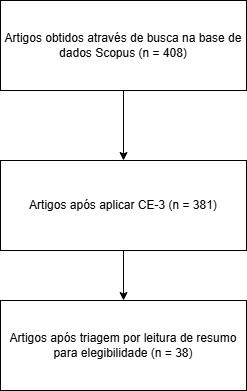
\includegraphics[width=.3\linewidth]{images/seleção-dos-artigos-primários.png}
	\label{fig:seleção-dos-artigos-primários}
  \source{Autor (2024)}
\end{figure}

\section{Tabela com os artigos primários selecionados}\label{section:tabela-com-os-artigos-primarios-selecionados}

A Tabela \ref{tab:EstudosPrimariosSelecionados} contempla os artigos primários selecionados.

\begin{longtable}{|p{3in}|p{2in}|p{1in}|}
	\caption{Estudos primários selecionados}
	\label{tab:EstudosPrimariosSelecionados} \\
	\hline
	\textbf{Título} & \textbf{Autores (Ano de publicação)} \\
	\hline
	Quality of service modeling for green scheduling in Clouds & \citeonline{Guérout2014225} \\
	\hline 
	Evaluating impact of live migration on data center energy saving & \citeonline{Akiyama2015759} \\
	\hline 
	A cloud computing resource scheduling policy based on genetic algorithm with multiple fitness & \citeonline{Chen2012177} \\
	\hline 
	Reduce VM migration in bandwidth oversubscribed cloud data centres & \citeonline{Shahzad2015140} \\
	\hline 
	Traffic-aware virtual machine migration scheduling problem in geographically distributed data centers & \citeonline{Teyeb2016798} \\
	\hline
	A computation- Network-Aware energy optimization model for virtual machines allocation & \citeonline{Canali201743} \\
	\hline
	Heuristic algorithms for energy and performance dynamic optimization in cloud computing & \citeonline{Guo20171335} \\
	\hline
	Carbon efficient VM placement and migration technique for green federated cloud datacenters & \citeonline{Wadhwa20142297} \\
	\hline
	Dynamic Virtual Machine migration algorithms using enhanced energy consumption model for green cloud data centers & \citeonline{Huang2014902} \\
	\hline
	Dynamic resource management using virtual machine migrations & \citeonline{Mishra201234} \\
	\hline
	Energy-Efficient Thermal-Aware Autonomic Management of Virtualized HPC Cloud Infrastructure & \citeonline{Rodero2012447} \\
	\hline
	Live migration of multiple virtual machines with resource reservation in cloud computing environments & \citeonline{Ye2011267} \\
	\hline
	Hybrid soft computing approach for energy efficiency in cloud computing & \citeonline{Jasuja2016} \\
	\hline
	Service-Oriented Virtual Machine Placement Optimization for Green Data Center & \citeonline{Tseng2015556} \\
	\hline
	Online virtual machine migration for renewable energy usage maximization in geographically distributed cloud data centers & \citeonline{Khosravi2017} \\
	\hline
	Type-aware virtual machine management for energy efficient cloud data centers & \citeonline{Al-Dulaimy2018185} \\
	\hline
	Live Migration for Multiple Correlated Virtual Machines in Cloud-Based Data Centers & \citeonline{Sun2018279} \\
	\hline
	An algorithm for network and data-aware placement of multi-tier applications in cloud data centers & \citeonline{Ferdaus201765} \\
	\hline
	Energy efficient temporal load aware resource allocation in cloud computing datacenters & \citeonline{Vakilinia2018} \\
	\hline
	Challenges in green computing for energy saving techniques & \citeonline{More201773} \\
	\hline
	PAPSO: A power-aware VM placement technique based on particle swarm optimization & \citeonline{Ibrahim202081747} \\
	\hline
	Energy aware virtual machine scheduling in data centers & \citeonline{Qiu2019} \\
	\hline
	A Strategy for Live Migration of Virtual Machines in a Cloud Federation & \citeonline{Addya20192877} \\
	\hline
	Memory-aware resource management algorithm for low-energy cloud data centers & \citeonline{Liang2020329} \\
	\hline
	VMSAGE: A virtual machine scheduling algorithm based on the gravitational effect for green Cloud computing & \citeonline{Xu201987} \\
	\hline
	Energy-aware virtual machine allocation and selection in cloud data centers & \citeonline{DineshReddy20191917} \\
	\hline
	An Energy-Aware Combinatorial Virtual Machine Allocation and Placement Model for Green Cloud Computing & \citeonline{Gamsiz202118625} \\
	\hline
	An approach toward design and development of an energy-aware VM selection policy with improved SLA violation in the domain of green cloud computing & \citeonline{Mandal20207374} \\
	\hline
	An Energy-Efficient Dynamic Resource Management Approach Based on Clustering and Meta-Heuristic Algorithms in Cloud Computing IaaS Platforms: Energy Efficient Dynamic Cloud Resource Management & \citeonline{AskarizadeHaghighi20191367} \\
	\hline
	Energy and carbon-aware initial VM placement in geographically distributed cloud data centers & \citeonline{Khodayarseresht2023} \\
	\hline
	VM Scheduling for Efficient Dynamically Migrated Virtual Machines (VMS-EDMVM) in Cloud Computing Environment & \citeonline{Supreeth20221892} \\
	\hline
	A Service Sustainable Live Migration Strategy for Multiple Virtual Machines in Cloud Data Centers & \citeonline{Satpathy2021} \\
	\hline
	Preserving Resource Handiness and Exigency-Based Migration Algorithm (PRH-EM) for Energy Efficient Federated Cloud Management Systems & \citeonline{Karthikeyan2023} \\
	\hline
	Power efficient virtual machine placement in cloud data centers with a discrete and chaotic hybrid optimization algorithm & \citeonline{Gharehpasha20211293} \\
	\hline
	MECpVmS: an SLA aware energy-efficient virtual machine selection policy for green cloud computing & \citeonline{Mandal2023651} \\
	\hline
\end{longtable}

\section{Análise descritiva}\label{section:analise-descritiva}

Através da Figura \ref{fig:artigos-por-ano} é possivel perceber que o interesse científico pelo assunto, desde que surgiu, é constante.
\begin{figure}[htbp]
	\centering
	\caption{Distribuição dos artigos selecionados no tempo}
		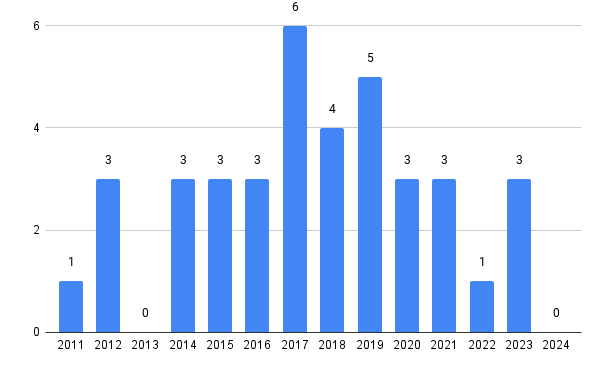
\includegraphics[width=\linewidth]{images/artigos-por-ano.png}
	\label{fig:artigos-por-ano}
  \source{Autor (2024)}
\end{figure}

A maior parte dos artigos selecionados foram publicados em periódicos, conforme mostra a Figura \ref{fig:local-de-publicação-do-artigo}.
\begin{figure}[htbp]
	\centering
	\caption{Local de publicação dos artigos selecionados}
		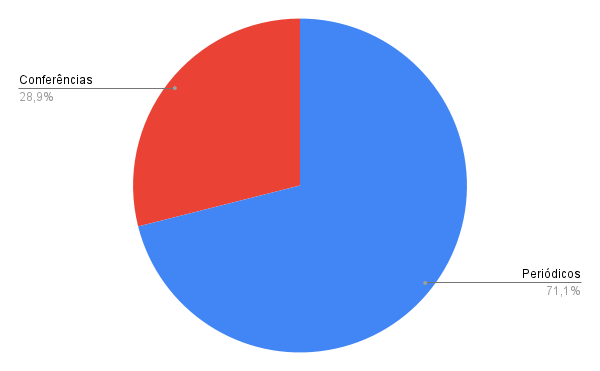
\includegraphics[width=\linewidth]{images/local-de-publicação-do-artigo.png}
	\label{fig:local-de-publicação-do-artigo}
  \source{Autor (2024)}
\end{figure}

\end{apendicesenv}
% ---


% ----------------------------------------------------------
% Anexos
% ----------------------------------------------------------

% ---
% Inicia os anexos
% ---
\begin{anexosenv}

% Imprime uma página indicando o início dos anexos
%\partanexos

\end{anexosenv}

%---------------------------------------------------------------------
% INDICE REMISSIVO
%---------------------------------------------------------------------
%%%%%MF\phantompart
%%%%%MF\printindex
%---------------------------------------------------------------------

\end{document}
